\chapter{Background}
\label{cha:background}

In this thesis, we will analyze in detail the behavior of an LLM as an agent within
a controlled environment.

Before presenting all the work carried out in detail, this chapter aims to
provide a comprehensive explanation of all the theoretical foundations necessary
to understand the steps presented in the following chapters. Starting from a brief
introduction of Artificial Intelligence just to define the boundaries in which we
are working, we will move to the core concepts. In particular, we want to
highlight what an LLM is and how it works, with a special focus on the Attention
mechanism and how the uncertainty of an LLM can be calculated. This will serve
as a basis for correctly interpreting the results analyzed in Section
\ref{cha:results_discussion}.

There will also be a broader discussion on agents in a strict sense and "LLM agents"
to better show the difference between our implementation and what is currently
being discussed over the media.

To better define the context of this thesis, we will examine the main alternative
approaches to solving a logistical problem currently studied in the literature.

\section{Artificial Intelligence}
\label{sec:artificial_intelligence}

Right now in the media, AI is being used as a synonym for Large Language Models.
However, AI is a broader concept that includes many techniques and methodologies.

\#\# Summary of different kind of AI ending with Generative Models end with NLP
history

\section{Large Language Models - LLMs}
\label{sec:large_language_models_llms}

\#\# LLMs are generative models released with the paper "Attention is All You
Need"

\subsection{LLMs' Uncertainty}
\label{sub:llms_uncertainty}

Understanding the uncertainty of an LLM is crucial to correctly interpret the text
it generates. If we ask for a yes/no question, it would make a different impact on
us reading "Yes" or "Yes - Uncertainty 49\%". Moreover, this would let us get
some kind of explainability behind these complex and opaque systems.

\#\# cite Hallucinations

\section{Agents}
\label{sec:agents}

% \begin{figure}[h!]
%   \label{fig:agent_scheme}
%   \centering
%   \includegraphics[width=.3333\textwidth]{images/Agent_Scheme.png}
%   \caption{Agent Scheme}
%   { Source: redesign of a scheme in \cite{wooldridge2002multiagent}}
% \end{figure}

As widely explained in the book "An Introduction to Multiagent Systems"
\cite{wooldridge2002multiagent}, we can summarize the definition of an agent as an
autonomous entity that perceives its environment through sensors and acts upon it
through effectors, making decisions based on its perceptions and objectives in
order to achieve specific goals.

This definition highlights several key aspects of agents:
\begin{itemize}
  \item Autonomy: Agents operate without direct human intervention, controlling their
    own actions.

  \item Perception and Action: They interact with the environment via sensors (perception)
    and effectors (action execution).

  \item Decision-making: Agents select actions based on their internal model, goals,
    and the state of the environment.

  \item Non-determinism and Adaptability: Since environments are generally non-deterministic,
    agents must be prepared for uncertainty and potential failures in action execution.

  \item Preconditions and Constraints: Actions are subject to certain conditions
    that must be met for successful execution.
\end{itemize}

Thus, an agent's fundamental challenge is deciding which actions to perform in order
to best satisfy its objectives, given the constraints and uncertainties of its
environment.

\begin{figure}[h!]
  \centering
  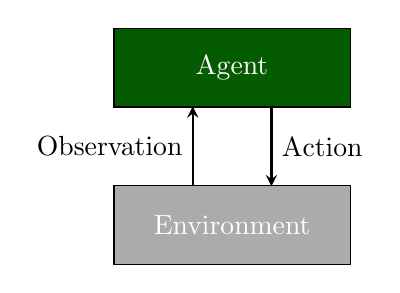
\begin{tikzpicture}[
    node distance=2cm, % Distance between nodes
  ]
    \node[
      rectangle,
      minimum width=3cm,
      minimum height=1cm,
      text centered,
      draw=black,
      fill={rgb,255:red,5; green,91; blue,0},
      text=white
    ] (agent) {Agent};
    \node[
      rectangle,
      minimum width=3cm,
      minimum height=1cm,
      text centered,
      draw=black,
      below of=agent,
      fill={rgb,255:red,171; green,171; blue,171},
      text=white
    ] (env) {Environment};

    % First arrow (Action) slightly shifted right
    \draw[thick, ->, >=stealth]
      (agent.south)
      ++(0.5,0) -- ++(0,-1)
      node[midway, right] {Action};

    % Second arrow (Observation) slightly shifted left
    \draw[thick, ->, >=stealth]
      (env.north)
      ++(-0.5,0) -- ++(0,1)
      node[midway, left] {Observation};
  \end{tikzpicture}
  \caption{Agent Scheme}
  { Source: redesign of a scheme in \cite{wooldridge2002multiagent}} \label{fig:agent_scheme}
\end{figure}

As shown in Figure \ref{fig:agent_scheme}, an agent is some entity that
perceives the environment and reacts to it. The environment can be anything from
a simple thermostat to a complex system like a self-driving car. The idea is
that the agent is able to react to a change in the environment and take actions
to achieve its goals.

We will analyze in detail the prompts and the choices in the Chapter
\ref{cha:data_collection} Section \ref{sec:prompts}, but to give an some kind of
help to align with the definition above, we can map some of its concept to what
this thesis will analyze:
\begin{itemize}
  \item Perception and Action: what the server sends about the current state of
    the environment can be seen as the perception of the agent, while the action
    it can take will be given in the prompt in a specific way.

  \item Decision-making: the decision-making process will be the generation of
    the text by the LLM, weighted by the uncertainty.

  \item Non-determinism and Adaptability: to emulate the non-determinism of the
    environment, the state received by the server will be used "raw" in the prompt,
    without any hard processing or parsing.

  \item Preconditions and Constraints: living in a "limited" map with a fixed
    number of cells, is itself a constraint the agent must consider.
\end{itemize}

\subsection{BDI Architecture}
\label{sub:bdi_architecture}

The Belief-Desire-Intention (BDI) architecture is a widely adopted framework in artificial
intelligence (AI) for modeling rational agents. It was formally developed by Rao
and Georgeff in 1995 \cite{bdi-icmas95} and has been implemented in several
architectures, including PRS (1987), dMARS (1998), JAM (1999), Jack (2001), and JADEX
(2005). BDI provides a structured approach to practical reasoning, allowing agents
to function effectively in dynamic and unpredictable environments.

\subsubsection{Core Components of BDI}
BDI agents operate based on three key components:
\begin{itemize}
  \item Belief: Represents the agent’s knowledge about the world, including past
    events and observations. Given the agent's local perception and limited
    computational resources, beliefs act as cached, imperfect information rather
    than absolute knowledge

  \item Desire (Goals): Defines the agent’s objectives or preferred end states, such
    as "desiring to graduate." Desires help in justifying why an agent takes
    specific actions and enable reasoning about goal interactions, particularly in
    failure recovery scenarios

  \item Intention: Represents the commitments of an agent toward achieving
    specific goals through selected plans. Intentions provide structure by ensuring
    persistence and internal consistency, allowing for incremental planning and
    adaptation in real-time. They also serve as a means of coordinating multiple
    agents in distributed systems.
\end{itemize}

\subsubsection{BDI in Practical AI Applications}

BDI has been extensively used in fields like robotics, automated planning, and
multi-agent systems. For instance, JADEX is a popular Java-based BDI framework
used in simulations and decision-making applications.

\section{State of the Art}
\label{sec:state_of_the_art}

A logistic problem is a typical problem in the field of AI, and there are
several approaches to solve it. In this section, we will analyze the main
alternatives to LLMs in the literature and highlight the core differences
between them and our approach.

\begin{quotation}
  This is a longer blockquote that may span multiple paragraphs. It is indented
  on both sides.
\end{quotation}

\begin{blockquote}
  This is another styled blockquote with a grey background.
\end{blockquote}

\subsection{PDDL Based Solution}

\subsubsection{Planning Domain Definition Language}

PDDL: pro (explainable, efficienza in ambienti limitati) e contro (time intensive,
non c'è adattamento, in un problema di dimensioni moderate è quasi impossibile usarlo
in real time)

Reinforcement Learning: pro (efficace, si può adattare all'ambiente che cambia) e
contro (convergenza ad un local minima nella reward function, no explainability,
costoso da allenare)

Agenti LLM (es. o1 di OpenAI): introduzione a temi emergenti come il Chain of
Thought, sottolineando come viene eseguito il reasoning e cosa differisce dal mio
approccio

Planning in LLM